\section{Archish S me20b032}
A Markov decision process can be described as a tuple $ \langle S, A, T, R \rangle $, where
\begin{itemize}
	\item $S$ is a finite set of states of the world;
	\item $A$ is a finite set of actions;
	\item $T : S \times A \rightarrow \Pi(S)$ is the \textit{state-transition function}, giving for each world state and agent action, a probability distribution over world states (we write $T(s,a,s^\prime)$ for the probability of ending in state $s^\prime$, gievn that the agent starts in state $s$ and takes action $a$);
	\item $R : S \times A \rightarrow \mathbb{R}$ is the reward function, giving the expected immediate reward gained by the agent for taking each action in each state (we write $R(s,a)$ for the expected reward for taking action $a$ in state $s$);
	\item A stationary policy, $ \pi : S \rightarrow A $, is a situation-action mapping that specifies, for each state, an action to be taken.
	\item $V_{\pi}(s)$ is the expected discounted sum of future reward for starting in state $s$ and executing policy $\pi$.
\end{itemize}

\begin{center}
\begin{figure}[h]
	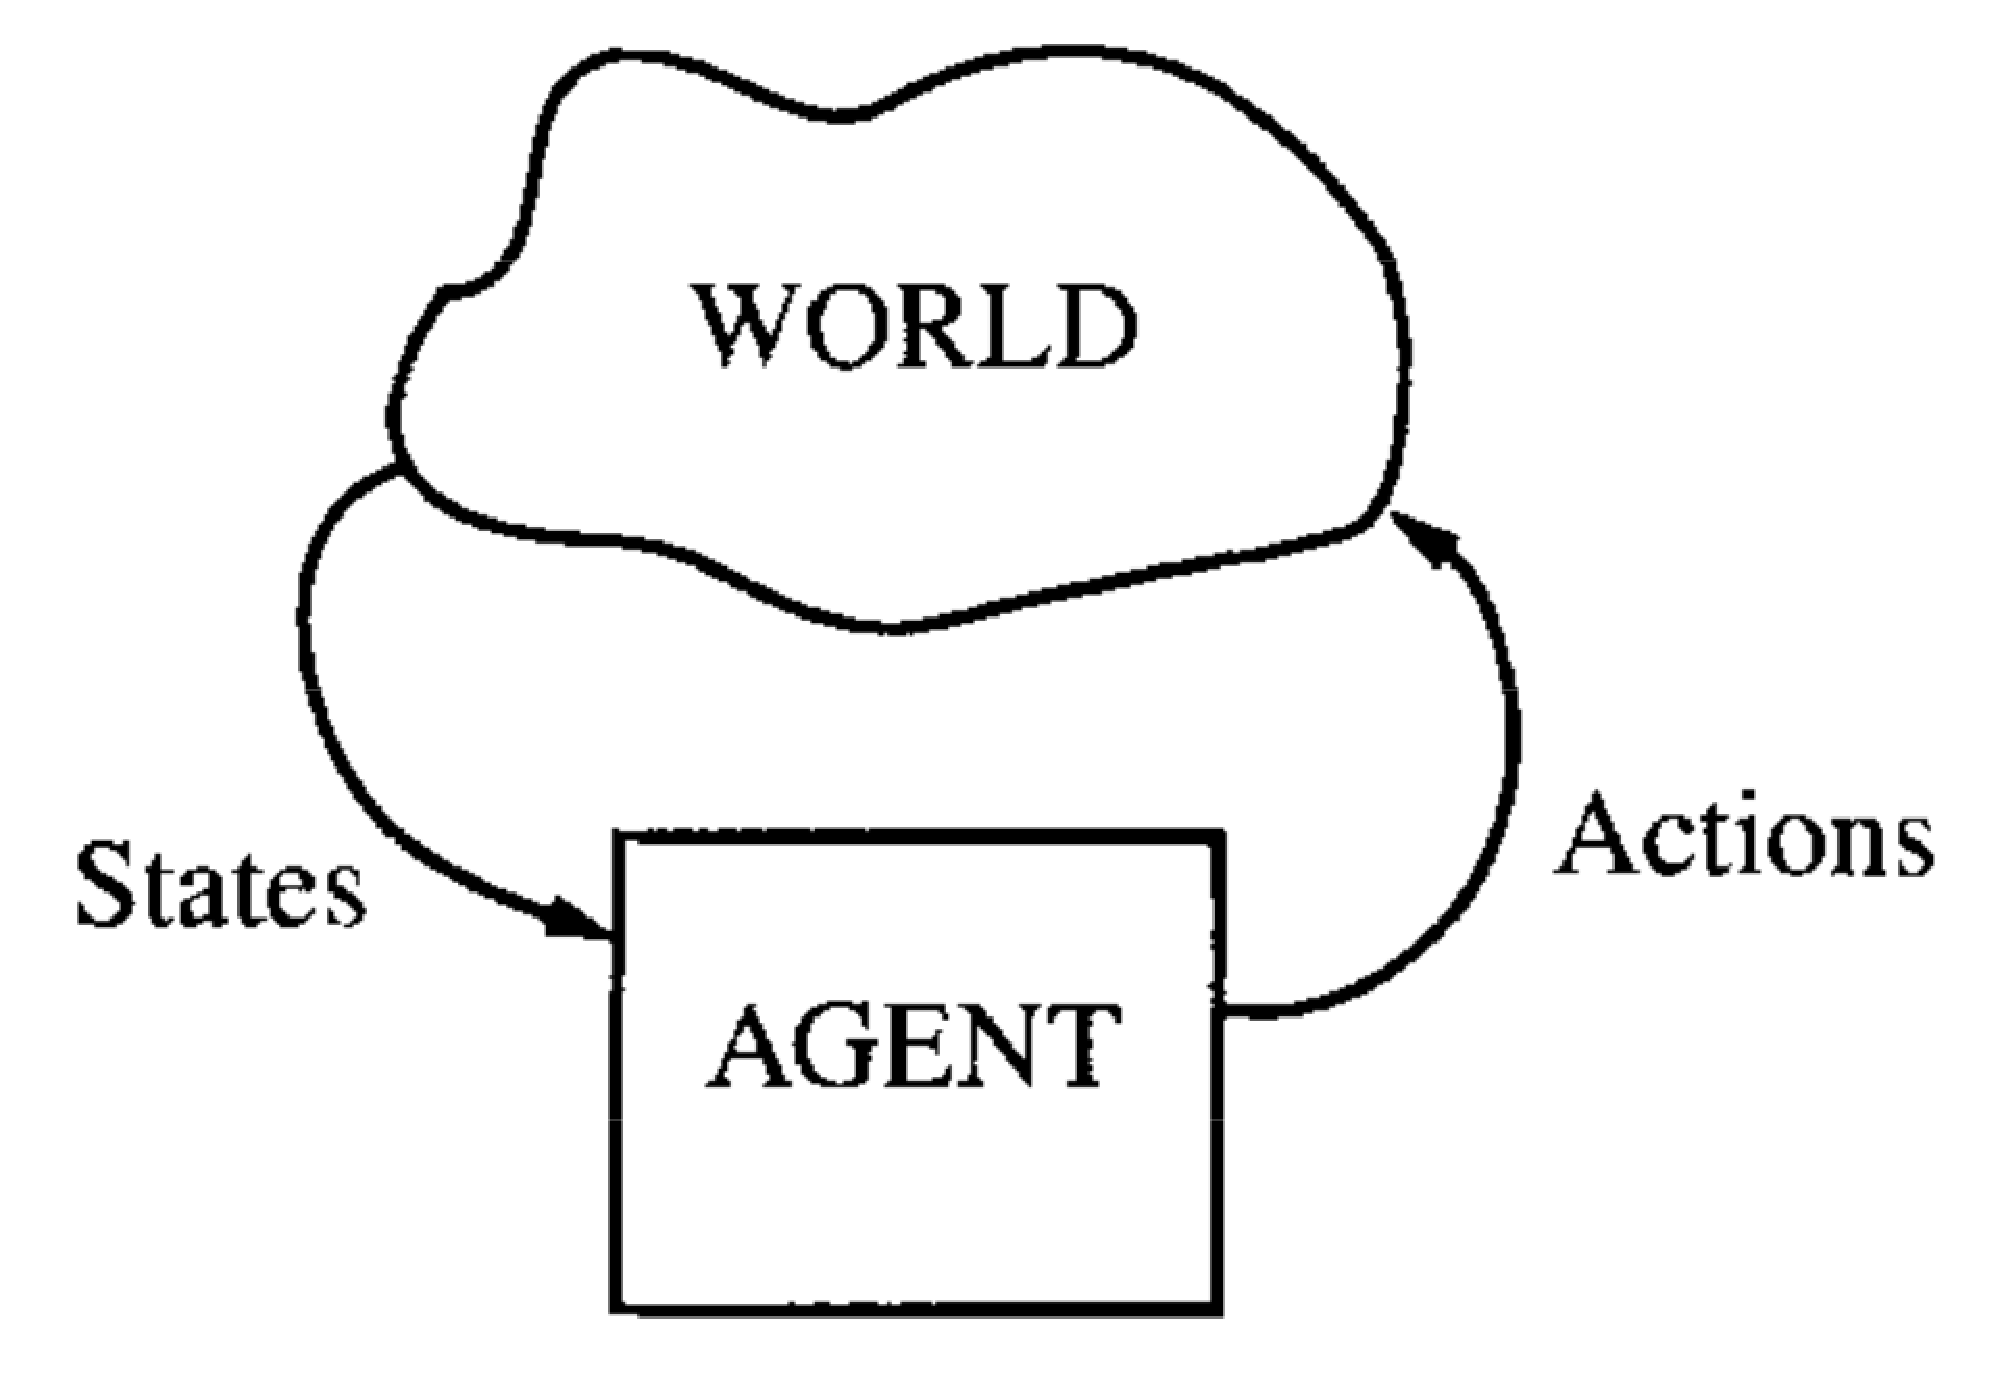
\includegraphics[width=\linewidth]{me20b032/me20b032.eps}
  	\caption{An MDP models the synchronous interaction between agent and world}
	\label{fig:MDP}
\end{figure}
\end{center}

In this model, as described by figure ~\ref{fig:MDP}, the next state and the expected reward depend only on the previous state and the action taken; even if we were to condition on additional previous states, the transition probabilities and the expected rewards would remain the same. This is known as the Markov property.

\begin{equation}
	V_{\pi}(s) = R(s,\pi(s)) + \gamma \sum_{s^\prime \in S} T(s, \pi(s), s^\prime) V_{\pi}(s^\prime)
	\label{eqn:ValueFunction}
\end{equation}
\\
Given the Value Funcition ~\ref{eqn:ValueFunction} a greedy policy with respect to that value function, $\pi_V$, is defined as 
\begin{equation}
	\pi_V(s) = \underset{a}{\mathrm{argmax}}\left[R(s,a) + \gamma \sum_{s^\prime \in S} T(s, \pi(s), s^\prime) V(s^\prime) \right]
\end{equation}